\chapter{Introduction}
Nonlinear systems\cite{sastry2013nonlinear}, as their name suggests, do not exhibit linear relationships between inputs and outputs. This inherent non-linearity means the system's response to changes in input can be complex and often unpredictable. In the real world, nearly all systems display some degree of nonlinearity. This nonlinearity can manifest in a variety of phenomena. For example, in systems with multiple inputs and outputs, the interdependencies between variables can become intricate, leading to coupling issues. Another frequent challenge is chaotic behavior\cite{ditto1995principles}\cite{oestreicher2007history}, where even minor alterations in initial conditions can lead to vastly different outcomes. Addressing these nonlinearities is crucial when managing control tasks, especially in real-world systems.

Achieving precise control over nonlinear systems\cite{iqbal2017nonlinear} has long been a primary focus in the field of control theory. While linear systems, often represented by linear differential equations, can typically be solved quickly and analytically, nonlinear equations representing nonlinear dynamics usually lack closed-form solutions\cite{struble2018nonlinear}. This necessitates the use of approximations and numerical methods. Efficiently and accurately executing these methods presents a central challenge in nonlinear control. Throughout history, control engineers have devised a wide range of strategies to manage these complex systems. The rise of robotics in recent decades has introduced new methods specifically tailored to address the challenges presented by nonlinearities.

\section{Motivation}
Robots are purposefully engineered as programmable mechanical structures, enabling them to perform a variety of tasks, either autonomously or under partial human oversight. These tasks include mobility, manipulation, and active interaction with their surroundings.

In the field of modern robotics, the mechanical systems are highly complex and nonlinear, posing significant challenges for precise and effective control. However, with the advancement of modern control methodologies and the increasing power of artificial intelligence, numerous innovative control approaches are emerging each year. Many products in modern robotics have achieved remarkable success, some well-known instances include quadruped robotics\cite{biswal2021development}, autonomous vehicles\cite{schwarting2018planning}, quadcopters\cite{luukkonen2011modelling}, and humanoid robots\cite{saeedvand2019comprehensive}.

\begin{figure}[H]
    \centering
    \begin{subfigure}[b]{0.45\textwidth}
        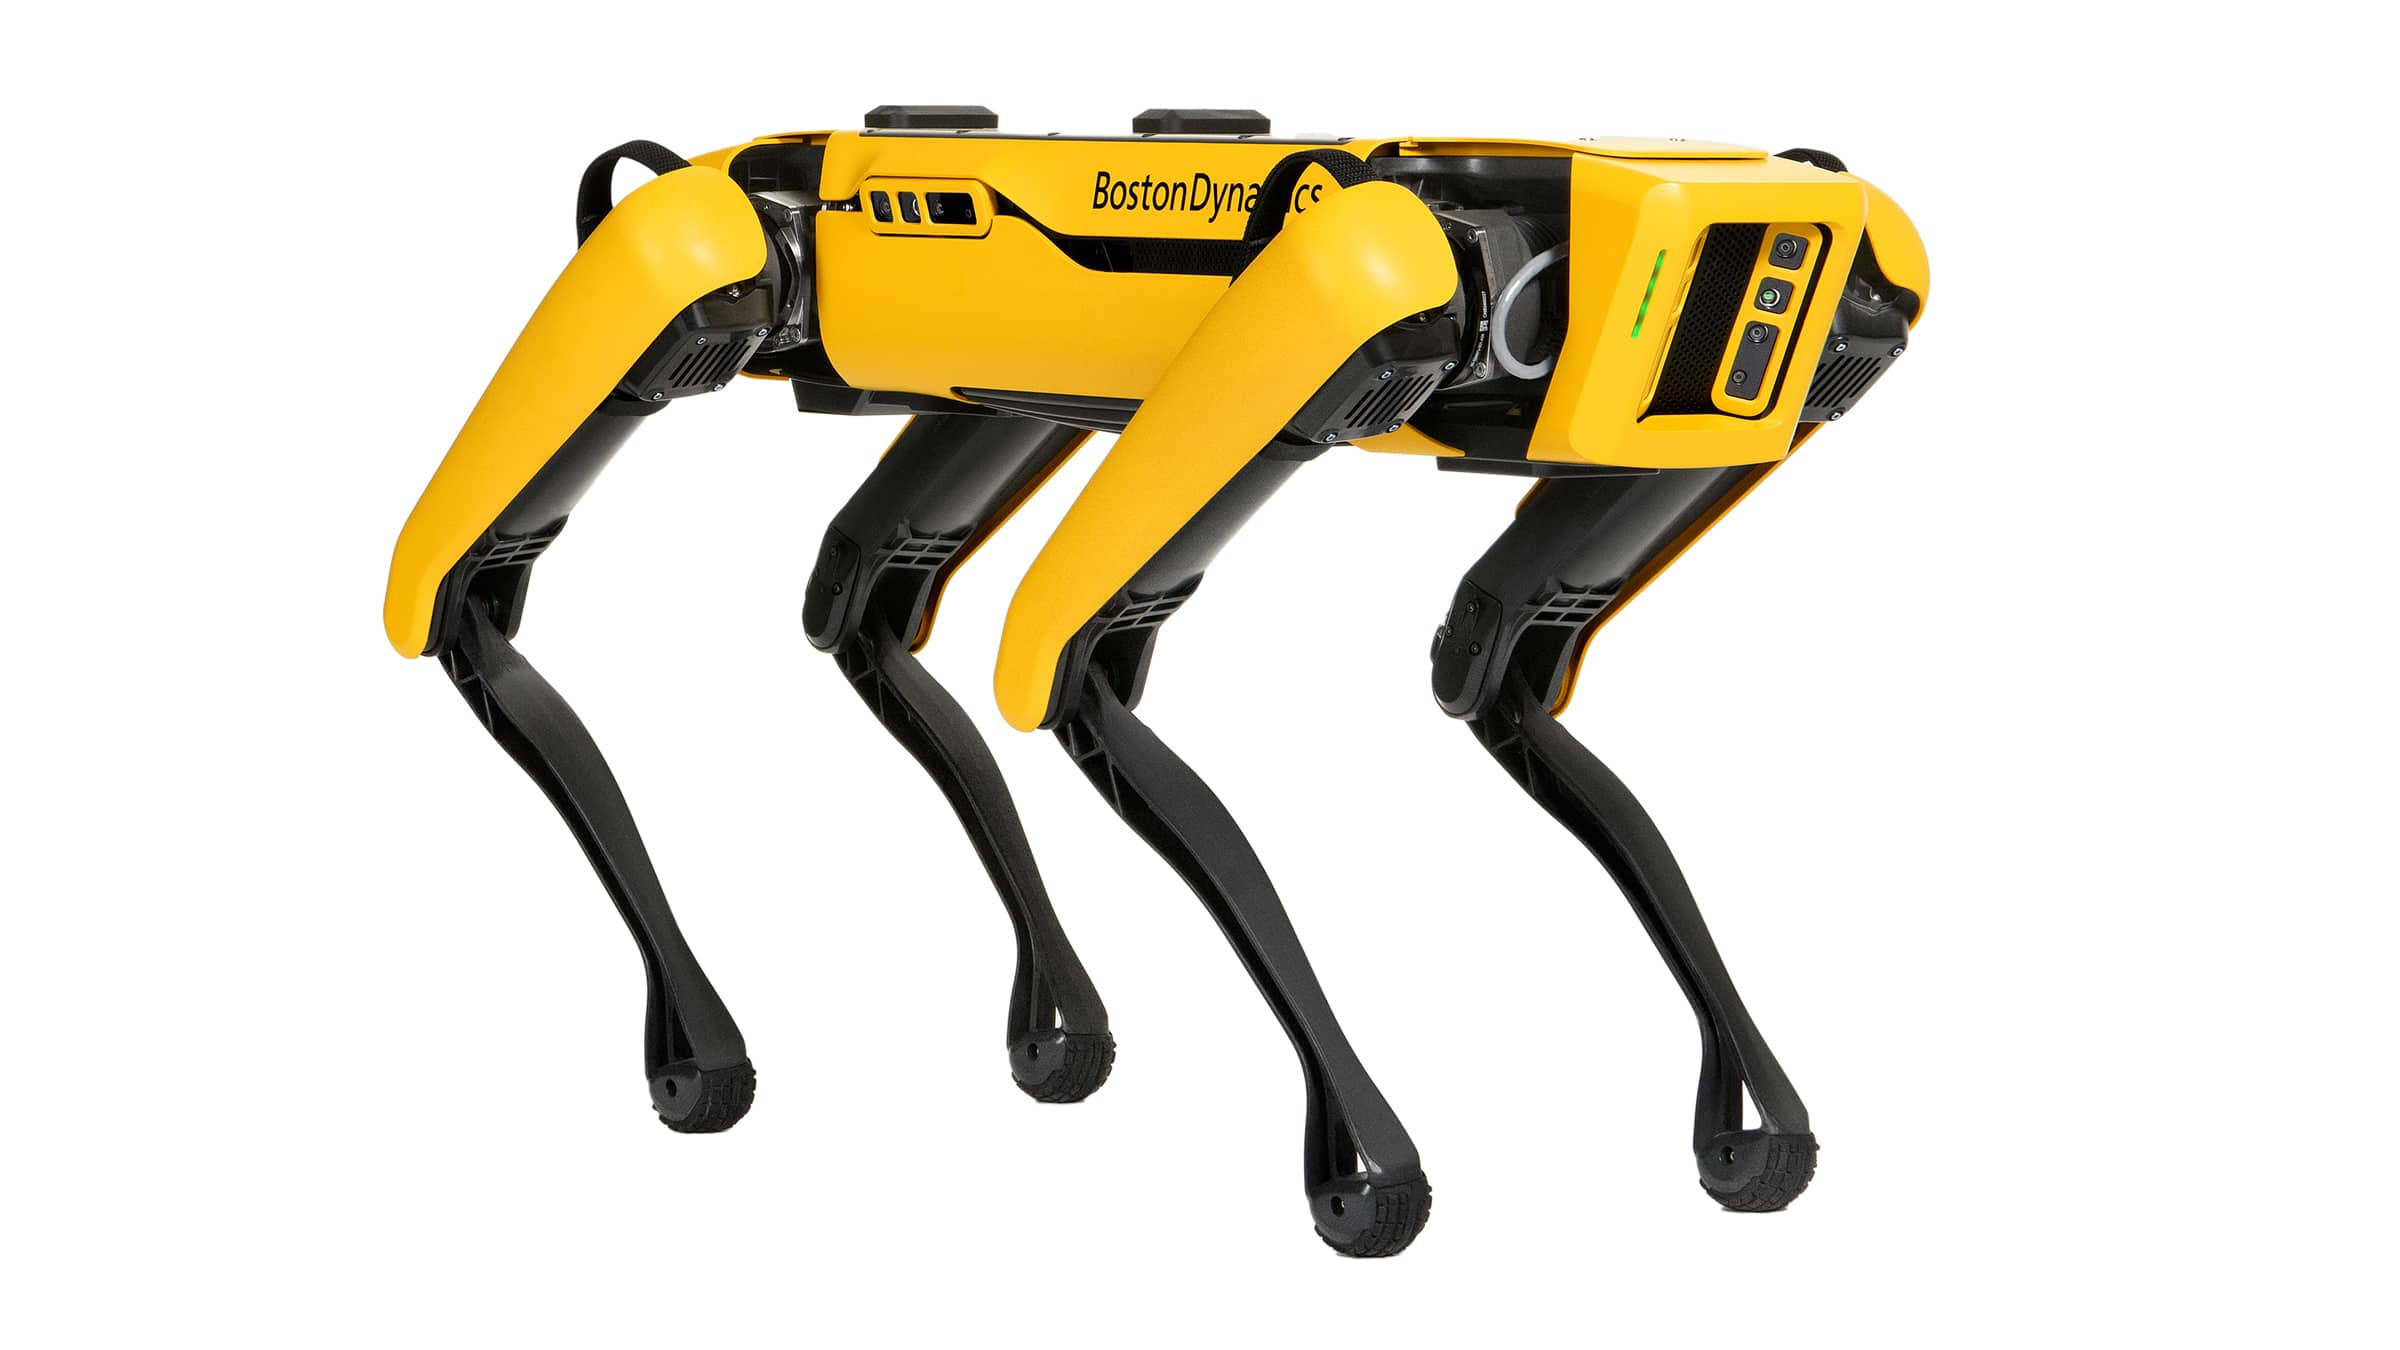
\includegraphics[width=\textwidth]{figures/quadruped.jpg}
        \caption{Quadruped}
        \label{fig:image1}
    \end{subfigure}
    \hfill
    \begin{subfigure}[b]{0.45\textwidth}
        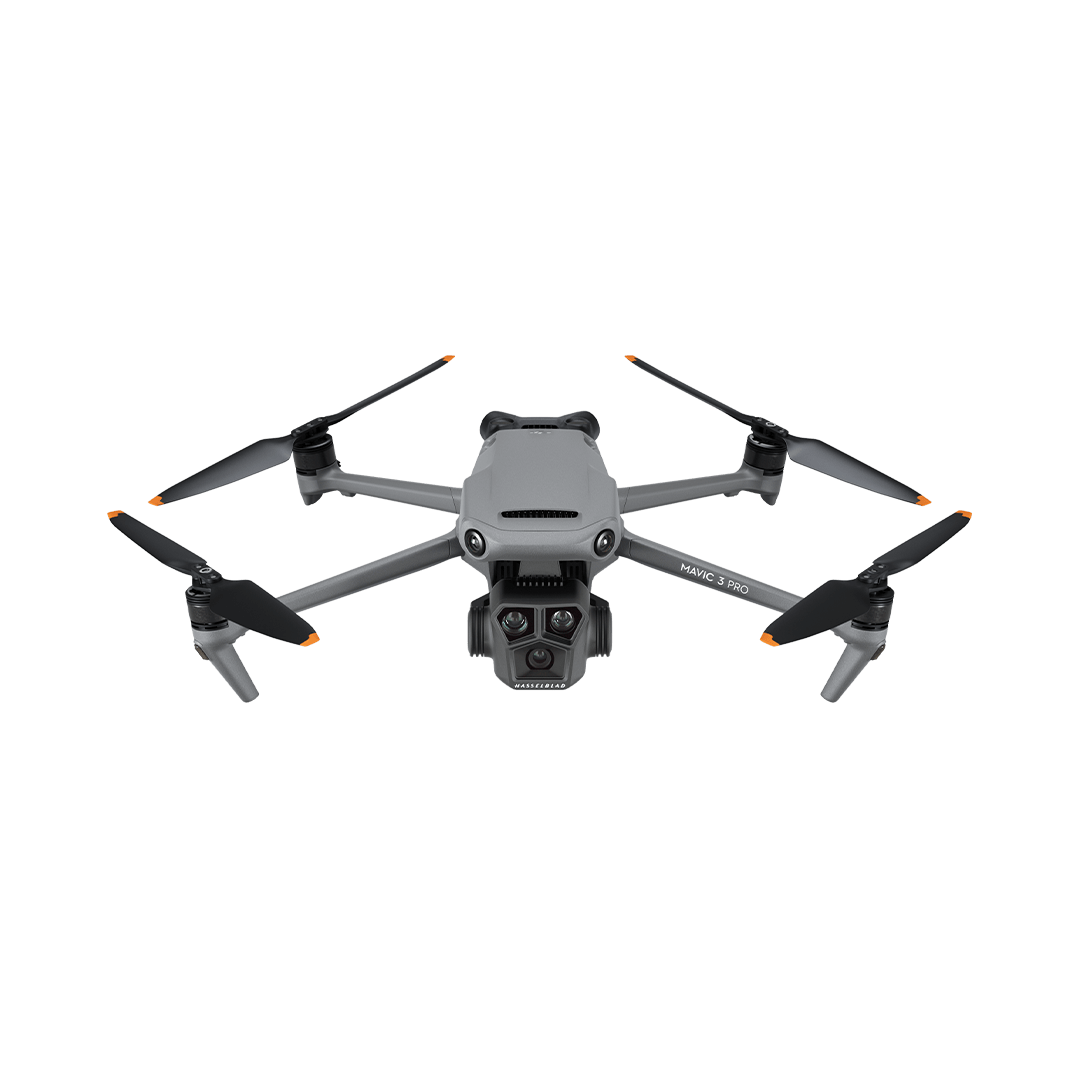
\includegraphics[width=\textwidth]{figures/quadcopter.png}
        \caption{Quadcopter}
        \label{fig:image2}
    \end{subfigure}

    \vspace{1em} % or use \bigskip or \medskip depending on the space you want

    \begin{subfigure}[b]{0.45\textwidth}
        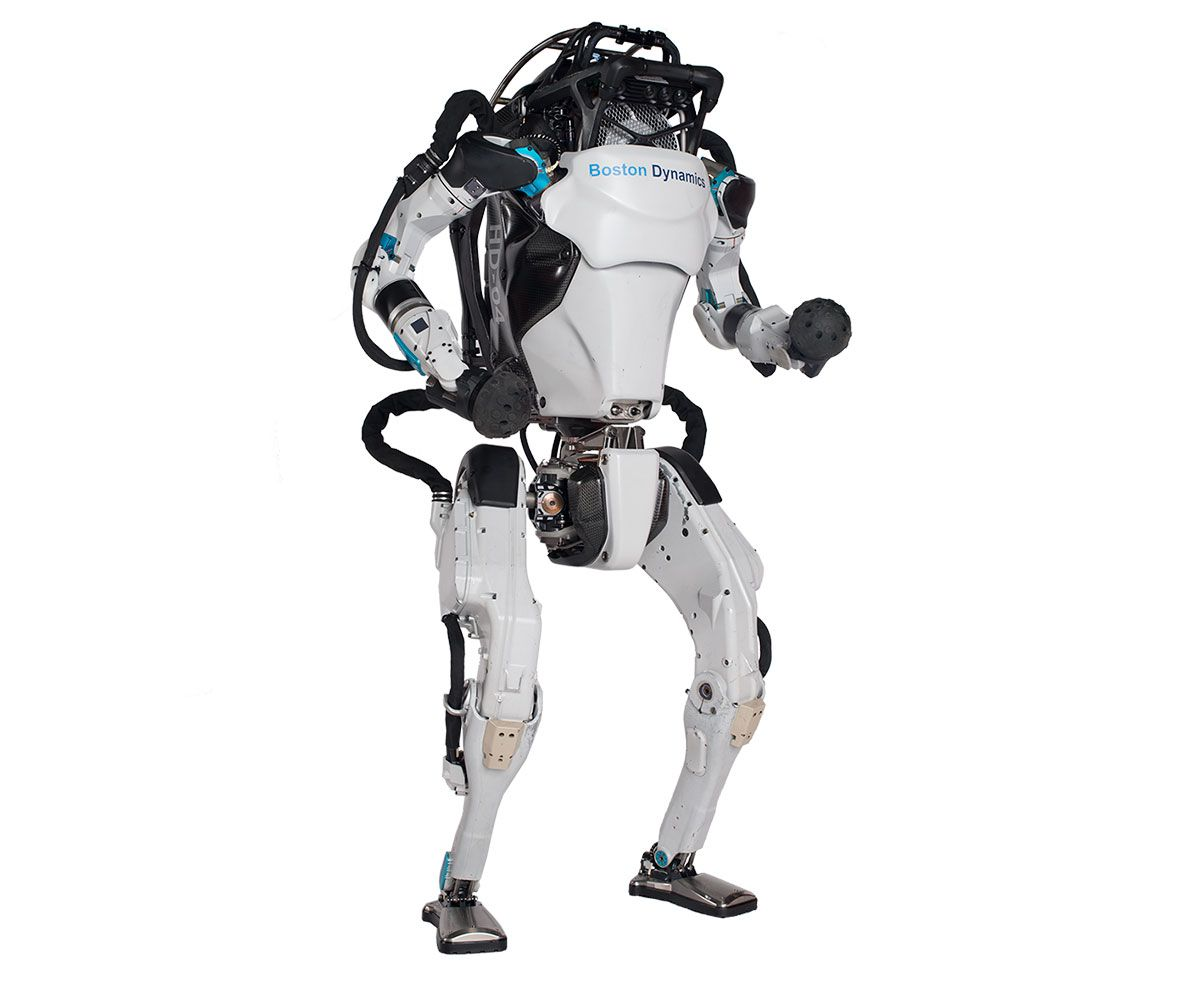
\includegraphics[width=\textwidth]{figures/humanoid.jpg}
        \caption{Humanoid}
        \label{fig:image3}
    \end{subfigure}
    \hfill
    \begin{subfigure}[b]{0.45\textwidth}
        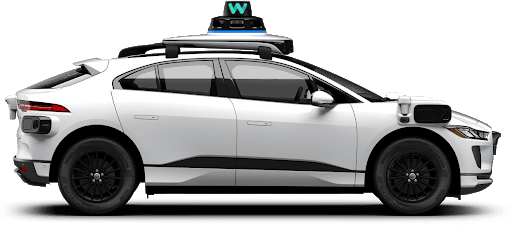
\includegraphics[width=\textwidth]{figures/waymo.png}
        \caption{Autonomous vehicle}
        \label{fig:image4}
    \end{subfigure}
    \caption{Four successful examples for controlling dynamic and nonlinear systems in the field of modern robotics}
    \label{fig:four_images}
\end{figure}

\subsection{Trajectory planning and tracking}
In the traditional control of complex systems such as robotics, which exhibit significant nonlinearity, it is crucial to employ dependable nonlinear control strategies to enhance motion capabilities. Typically, the procedure for planning intricate movements within these systems adheres to a two-phase method\cite{biagiotti2008trajectory}, encompassing trajectory planning and trajectory tracking. This structured approach ensures precision and stability in robotic system control.

Trajectory planning\cite{gasparetto2015path}\cite{gasparetto2012trajectory} involves calculating a smooth and feasible path for the robot to follow, aiming for a specific target position or operational point. A widely-used method in this stage is trajectory optimization\cite{betts1998survey}, which seeks to minimize a cost function accounting for travel time, energy consumption, and motion smoothness. Techniques such as gradient descent or genetic algorithms are often utilized for optimization, with adherence to constraints like maximum velocities and accelerations being a crucial aspect of the process.

Upon successful trajectory planning, the next step is trajectory tracking, which entails the use of control algorithms to guide the robot along the predetermined path. A feedback control approach is typically employed, continually monitoring the robot's position and adjusting control inputs as necessary. However, in real-world systems, external disturbances, uncertainties, and system limitations may lead to significant deviations from the planned trajectory. Therefore, ensuring accurate state estimation and implementing robust control strategies are imperative in feedback control to address these challenges.

In industrial robot control\cite{gasparetto2010optimal}, the practice typically involves dividing the control process into distinct phases of offline planning and execution. This segmentation is primarily due to the non-critical requirement for real-time responsiveness in such applications. Take, for instance, the planning phase, where an algorithm such as A* is employed to determine an optimal route based on a predefined task, navigating around obstacles and minimizing travel distance, which results in a set of discrete waypoints\cite{cui2011based}. Following this, cubic interpolation techniques are applied to these waypoints, crafting a smooth and continuous trajectory that the robot can realistically follow, ensuring both fluid motion and compliance with the robot's kinematic constraints\cite{bickley1968piecewise}. The process subsequently moves to the execution phase, where a robust and precise control strategy is implemented. This strategy is crucial as it guarantees the robot's meticulous adherence to the pre-established trajectory, maintaining both accuracy and reliability throughout the operation\cite{lynch2017modern}.

Yet, in dynamic domains like automotive and flight control, the demand for real-time responsiveness takes center stage. For example, Model Predictive Control (MPC)\cite{kouvaritakis2016model} stands as a prime illustration of this critical requirement, seamlessly integrating online trajectory planning and execution into a unified framework. It initiates the process by forecasting a series of future control actions as part of the planning phase. Subsequently, during execution, these control inputs are refined to minimize any discrepancies between the real-time system state and the intended trajectory, ensuring precise alignment. MPC excels in its ability to simultaneously create, optimize, and follow trajectories, all while dynamically adjusting in real-time to accommodate disturbances and uncertainties. This capability is vital for maintaining precise control and adaptability in fast-paced and complex environments.

The traditional trajectory generation and tracking approach, while effective for numerous systems, has its own set of limitations.
\begin{itemize}
    \item \textbf{Limited Adaptability:}
    Trajectory planning typically relies on predefined paths or trajectories, limiting adaptability to unforeseen changes or dynamic environments. If the environment changes significantly, the planned trajectory may no longer be optimal or even feasible.
        
    \item \textbf{Difficulty with Nonlinear Systems:}
    Trajectory planning struggles with highly nonlinear systems where the dynamics are hard to model accurately. Linearizing the system for planning purposes may lead to suboptimal or infeasible trajectories.
    
    \item \textbf{High Computational Demands:}
    Some trajectory planning algorithms can be computationally intensive, especially for high-dimensional or complex robotic systems. This computational demand becomes a drawback, particularly in real-time or time-critical applications.
\end{itemize}

Recognizing the limitations inherent in traditional trajectory generation and tracking methodologies is essential for fostering the development of more advanced and efficient strategies in trajectory planning and control. This insight becomes particularly crucial in contexts that require rapid responsiveness and a capacity to skillfully navigate unpredictable changes or dynamic environments.

\subsection{Reinforcement Learning Based Control}
Transitioning from a focus on predefined trajectories, reinforcement learning(RL)-based control presents an alternative framework.

Reinforcement learning(RL)\cite{sutton2018reinforcement} is a subset of machine learning centered on agents learning optimal behavior through trial-and-error interactions with their environment. Essentially, the agent makes sequential decisions, observes the outcomes of its actions, and receives feedback in the form of rewards or penalties. This feedback serves as a guiding mechanism, enabling the agent to evaluate the outcomes of its actions and adjust its policy accordingly to maximize cumulative rewards over time.

The mathematical framework that describes RL is the Markov Decision Process(MDP)\cite{puterman1990markov}, which provides a structured model for the decision-making problem. In an MDP, the agent's current state, available actions, potential next states, and the rewards associated with state-action transitions are all clearly defined. This structure ensures that the future state of the system depends only on the current state and the action taken, fulfilling the Markov property.

\begin{figure}[h]
    \centering
    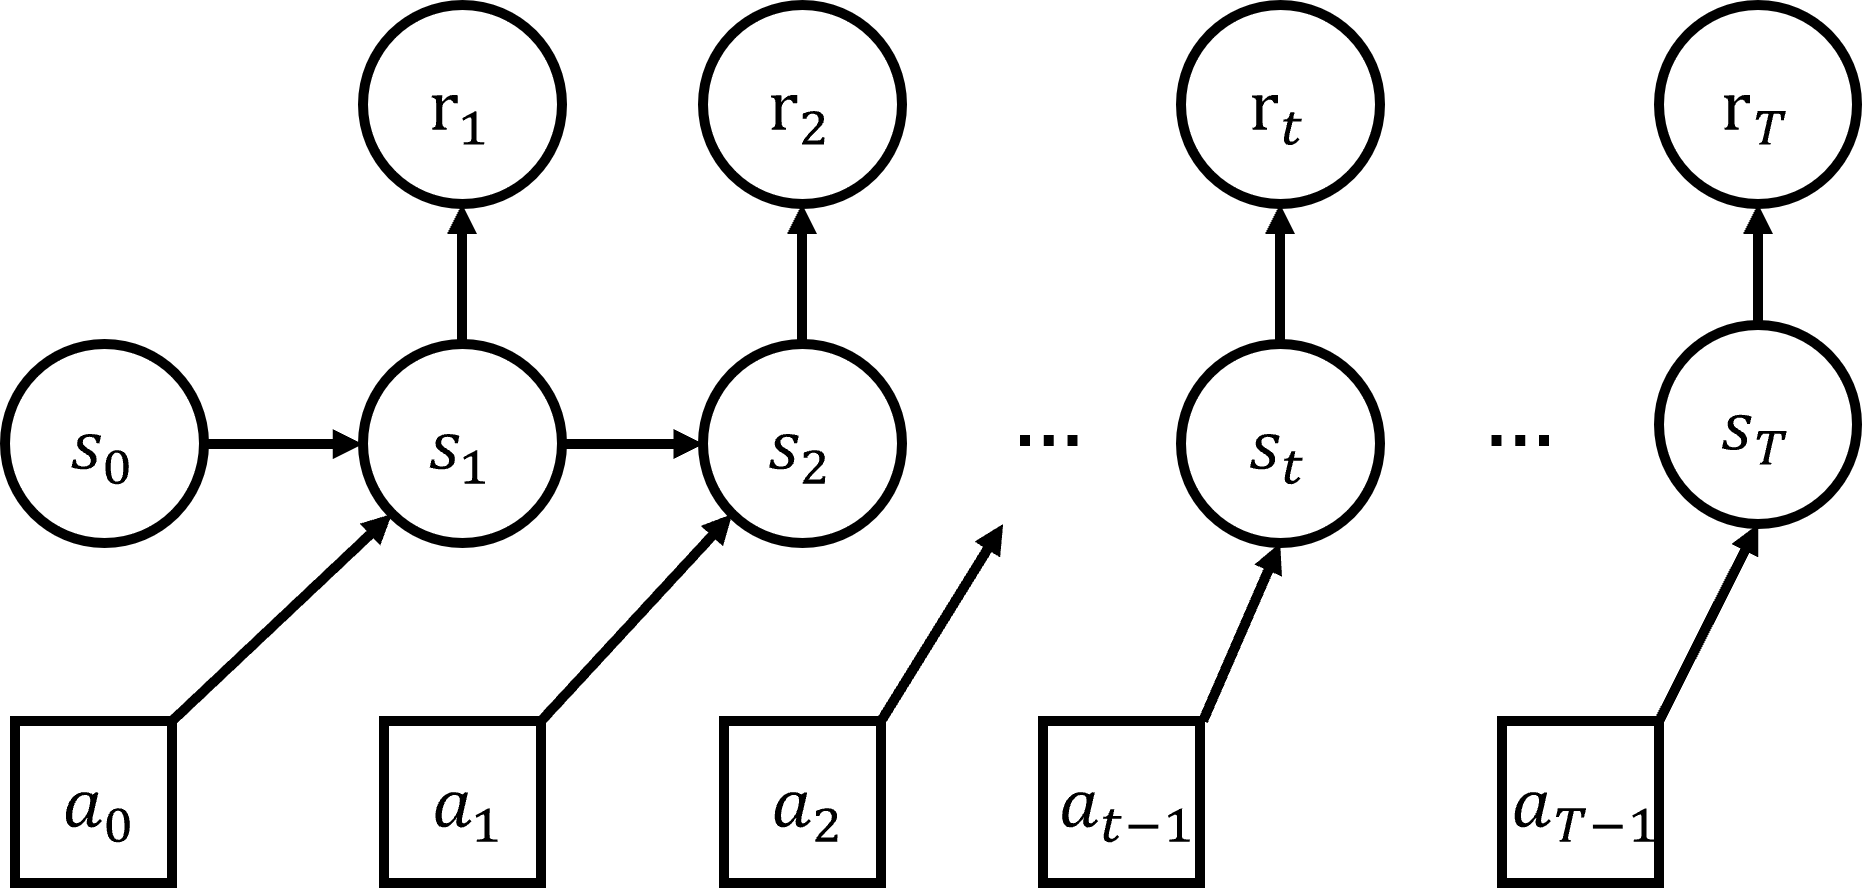
\includegraphics[width=0.8\textwidth]{figures/MDP.png}
    \caption{Markov decision process}
    \label{fig:mdp}
\end{figure}

The ultimate objective in RL is to find an optimal policy, a mapping from states to actions, that dictates the best action to take in each state to achieve maximum long-term rewards. The learning process is driven by the tuple \((s,a,r,s')\), representing the current state, action taken, received reward, and subsequent state. Over time, through exploration of the state-action space and exploitation of acquired knowledge, the agent refines its policy, converging towards optimal behavior.

A key challenge in RL is balancing exploration and exploitation. Exploration involves trying out different actions to discover their potential outcomes, essential for acquiring new knowledge. Exploitation, on the other hand, entails leveraging existing knowledge to make optimal decisions. Striking the right balance between these two strategies is crucial for the agent to effectively navigate its environment and learn from received rewards.

In the field of robotic control\cite{kober2013reinforcement}, the integration of reinforcement learning has become increasingly popular due to the numerous distinct advantages this combined approach offers:

\begin{itemize}
    \item \textbf{Adaptability and Flexibility:}
    RL allows systems to adapt and improve in dynamic environments. Its control policy evolves through accumulating new experiences and knowledge from interactions with the environment, making it highly adaptable to varying circumstances.

    \item \textbf{Reduced Dependency on Accurate Models:}
    In contrast to traditional control methods that depend on exact mathematical models, RL thrives without the necessity of a predetermined model, particularly when learning from real-world data. This feature is immensely beneficial in situations where the system dynamics are either intricate or not well understood, as RL refines its performance through direct interactions with the environment.

    \item \textbf{Effective Handling of Nonlinearities and High-Dimensional Systems:}
    RL excels at managing nonlinear systems and complex control tasks using neural network-based function approximation. This enables it to navigate high-dimensional input spaces and control intricate relationships between states and actions in complex scenarios.
\end{itemize}

Reinforcement learning distinguishes itself as a straightforward control method with high adaptability, setting itself apart from traditional trajectory generation and tracking techniques. While conventional methods frequently struggle with challenges such as limited adaptability, nonlinearity in systems, and intensive computational demands, reinforcement learning addresses these issues through direct interactions with the environment. It excels in unpredictable conditions and in managing complex, high-dimensional systems. This is largely attributed to its reduced dependency on accurately predefined dynamic models, ensuring robustness, effectiveness, and versatility across a wide range of applications.


\section{Problem setup}
In the realm of nonlinear systems, underactuated systems\cite{liu2013survey} present a particularly challenging class. These systems are characterized by having fewer control inputs than degrees of freedom, or their control inputs are constrained in some way. This characteristic makes them significantly more challenging to control when compared to fully actuated systems. What's intriguing is that a majority of robots and even natural organisms fall into the category of underactuated systems. Consequently, the study of underactuated mechanical systems' control holds universal relevance.

The concept of underactuated dynamics can be briefly introduced as follows. According to Newton's second law (\( F = ma \)), the dynamics that govern any mechanical system can be mathematically expressed as shown in Equation \ref{eq:nonlinear_dynamics_general_form}:

\begin{align}
    \ddot{q} = f(q, \dot{q}, u, t)
    \label{eq:nonlinear_dynamics_general_form}
\end{align}

In this equation, \( \ddot{q} \) represents acceleration, which is the second derivative of the variable \( q \), typically representing the position of the system. The function \( f(q, \dot{q}, u, t) \) describes how \( \ddot{q} \) depends on various parameters, including the state variables \( q \) and \( \dot{q} \), the control inputs \( u \), and the time \( t \).

The state of the system, denoted as \( x \) and represented as \( [q, \dot{q}]^T \), consists of two vectors: \( q \), which signifies positions, and \( \dot{q} \), which signifies velocities.

When dealing with control-affine systems, we can express the second-order differential equation in the following manner:

\begin{align}
    \ddot{q} = f_1(q, \dot{q}, t) + f_2(q, \dot{q}, t)u
    \label{eq:nonlinear_dynamics_control_form}
\end{align}

In this equation, \( f_1(q, \dot{q}, t) \) corresponds to one part of the function that affects \( \ddot{q} \), while \( f_2(q, \dot{q}, t) \) represents another part that interacts with the control input \( u \).

In the context of a controlled dynamical system, as described by Equation \ref{eq:nonlinear_dynamics_control_form}, we evaluate the condition of underactuation at specific states \([q, \dot{q}]^T\) at time \(t\). Underactuation can be identified through two distinct scenarios:

\begin{itemize}
 \item \textbf{Case 1:}
 
 The system is classified as underactuated at a particular state if the rank of the matrix \([f_2(q, \dot{q}, t)]\) is less than the dimension of \(q\). This condition is expressed as:
 
 \begin{align}
    \text{rank}[f_2(q, \dot{q}, t)] < \text{dim}[q]
\end{align}
 
 \item \textbf{Case 2:} 
 
 Alternatively, underactuation may also arise even when \(f_2\) is full rank, provided there are additional constraints on the control inputs. For instance, if constraints such as \(|\mathbf{u}| \leq 1\) limit the control inputs, the system's controllability can still be restricted, resulting in underactuation.
\end{itemize}

These principles are explained in the work by Russ Tedrake\cite{tedrake2022underactuated}.

A well-discussed example of underactuated control is found in the double pendulum—a simple setup consisting of two links connected by two rotational joints. These joints include the shoulder joint, which is directly connected to the world frame, and the elbow joint, situated between the two links. The end effector is located at the tip of the second link. Active control is achieved by attaching motors to the shoulder and elbow joints. In the domain of underactuated control, if the shoulder joint is actuated, the setup is referred to as a pendubot (see Figure \ref{pendubot_explained}). Conversely, if the elbow joint is actuated, it is known as an acrobot (see Figure \ref{acrobot_explained}).

\begin{figure}[htbp]
    \centering
    \begin{subfigure}[b]{0.2\textwidth}
        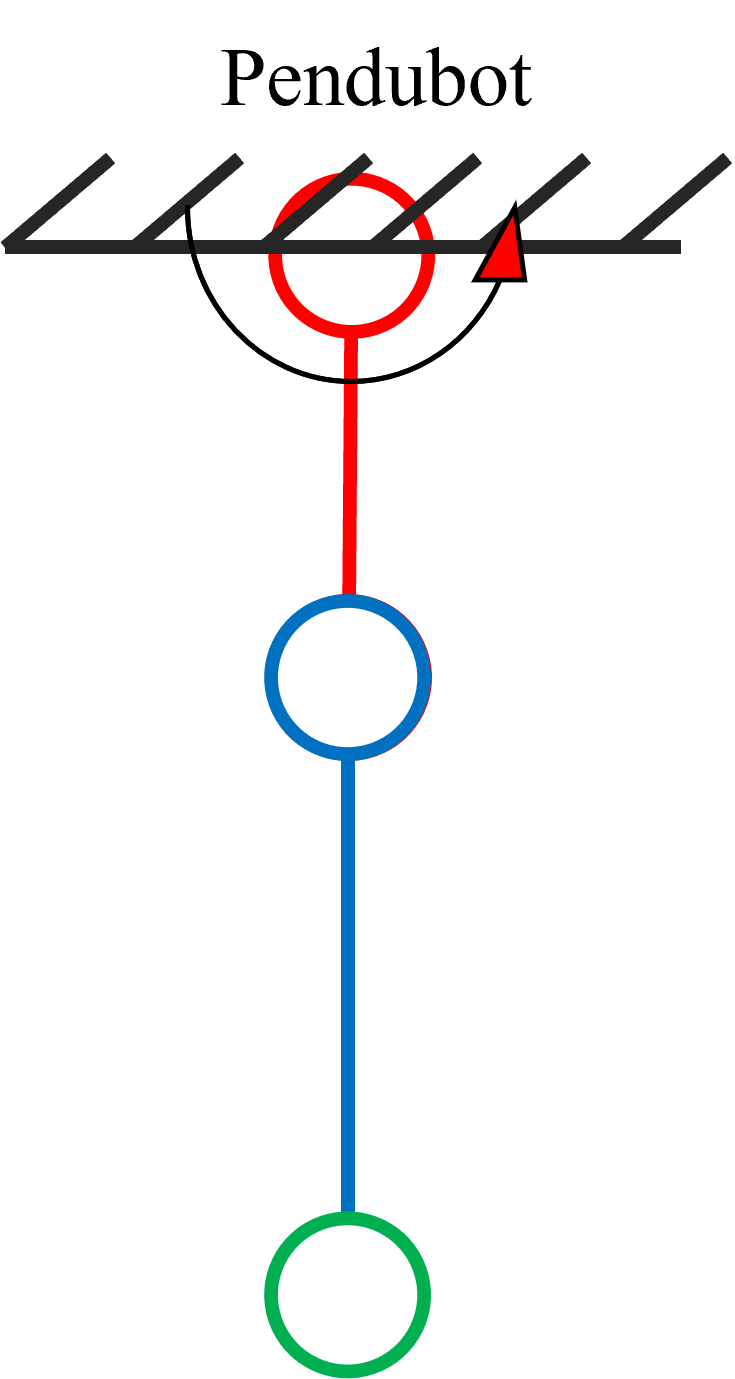
\includegraphics[width=\textwidth]{figures/pendubot_explained.png}
        \caption{Pendubot setup}
        \label{pendubot_explained}
    \end{subfigure}
%     \hfill
    \begin{subfigure}[b]{0.2\textwidth}
        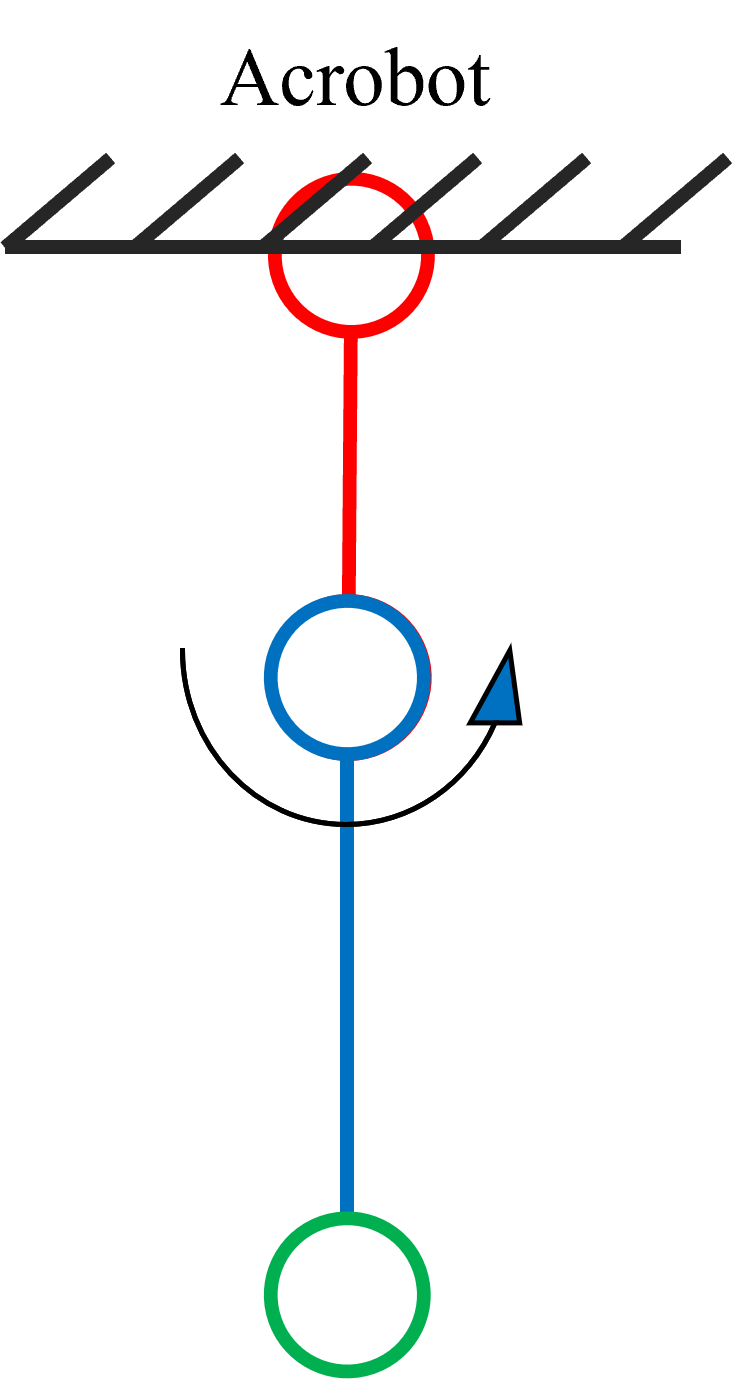
\includegraphics[width=\textwidth]{figures/Acrobot_explained.png}
        \caption{Acrobot setup}
        \label{acrobot_explained}
    \end{subfigure}
    \caption{Two variations of underactuated double pendulum}
\end{figure}

Despite its simple configuration, the system exhibits highly nonlinear and chaotic behavior\cite{shinbrot1992chaos}. The double pendulum setup presents two classic tasks: swing-up and stabilization around the highest point. Research on swing-up and stabilization of the double pendulum can be traced back to the 1990s\cite{yamakita1995robust}, and it continues to be a crucial testbed for validating the effectiveness of newly designed control algorithms\cite{xin2004new}\cite{zheng2006control}\cite{albahkali2009swing}.

Our project's objective is to develop a reinforcement learning-based control method suitable for underactuated control of the double pendulum system, specifically addressing swing-up and stabilization tasks. To evaluate the efficacy of this control method, we conduct both simulations and real system experiments.


\section{Contribution}
In this paper, the main contribution is as follows: An effective control strategy has been developed to achieve two key objectives with the double pendulum. The first task involves swinging the double pendulum from its lowest point to its highest point. The second task is to ensure stability at the highest point for an extended time period.

To address the swing-up task, a well-known model-free reinforcement learning algorithm called Soft Actor-Critic (SAC) was utilized\cite{haarnoja2018soft}. This algorithm enabled the training of a policy capable of reaching the Region of Attraction (RoA) of a continuous-time linear quadratic regulator (LQR) controller\cite{lehtomaki1981robustness}. Once the RoA is reached by the system, a seamless transition to the LQR controller is made to maintain stability around the highest point.

\section{Content}
This thesis comprises six chapters, namely: introduction, state of the art, methodology, agent training and experiments in a simulation environment, experiments on real hardware, discussion, and future work. At the end of Chapter One, the content of the following chapters is outlined below.

\begin{itemize}
  \item \textbf{Chapter 2: State of the Art}:
    \begin{itemize}
      \item This chapter begins by providing an explanation of the fundamental theories related to double pendulum dynamics. It is followed by an overview of recent advancements in the field of robotic control, with a specific focus on learning-based control methods.
    \end{itemize}
  
  \item \textbf{Chapter 3: Methodology}:
    \begin{itemize}
      \item This chapter delves into the methodology, covering fundamental aspects of reinforcement learning, with a specific focus on the SAC algorithm. It explains the reward function used for training, the training procedure, and introduces the concept of the LQR controller and the composition of the combined controller.

      \item Additionally, we introduce the evaluation metrics used to assess the performance and robustness of the newly designed control strategies in both simulated environments and real-world experiments.
    \end{itemize}

  
  \item \textbf{Chapter 4: Agent training and experiments in simulation environment}:
    \begin{itemize}
      \item In this chapter, we present the results obtained from simulations, showcasing the performance and behavior of the designed control strategy.
    \end{itemize}
  
  \item \textbf{Chapter 5: Experiments on real hardware}:
    \begin{itemize}
      \item This chapter reports the outcomes of experiments conducted on the hardware, providing insights into our approach to addressing the sim2real transfer problem.
    \end{itemize}
  
  \item \textbf{Chapter 6: Discussion and Future Work}:
    \begin{itemize}
      \item The final chapter engages in a discussion about the obtained results and explores potential future research and development directions.
    \end{itemize}
\end{itemize}


\cleardoublepage
